\documentclass[12pt,a4paper]{article}

% ─── Page Layout ───────────────────────────────────────────────────────────────
\usepackage[a4paper, margin=0.8in, headheight=14pt]{geometry}

% ─── Fonts (XeLaTeX) ───────────────────────────────────────────────────────────
\usepackage{fontspec}
\usepackage{unicode-math}
\setmainfont{TeX Gyre Pagella}
\setmonofont[Scale=0.88]{TeX Gyre Cursor}
\setmathfont{Latin Modern Math}

% ─── Packages ──────────────────────────────────────────────────────────────────
\usepackage{xcolor}
\usepackage{colortbl}
\usepackage{titlesec}
\usepackage{enumitem}
\usepackage{tabularx}
\usepackage{booktabs}
\usepackage{array}
\usepackage{amsmath}
\usepackage{tikz}
\usetikzlibrary{shapes.geometric, arrows.meta, positioning, calc, fit, decorations.pathreplacing, patterns}
\usepackage{tcolorbox}
\tcbuselibrary{skins, breakable}
\usepackage{hyperref}
\usepackage{fancyhdr}
\usepackage{graphicx}
\usepackage{microtype}
\hyphenpenalty=10000
\exhyphenpenalty=10000
\sloppy
\usepackage{caption}
\usepackage{setspace}
\usepackage{multirow}
\usepackage{tocloft}

% ─── Q&A helper ────────────────────────────────────────────────────────────────
\newcommand{\Q}[1]{\textbf{#1}\par\noindent\ignorespaces}

% ─── Colour Palette ────────────────────────────────────────────────────────────
\definecolor{myred}{RGB}{196,30,58}
\definecolor{mydark}{RGB}{30,30,50}
\definecolor{mygreen}{RGB}{14,120,80}
\definecolor{myteal}{RGB}{0,130,140}
\definecolor{myamber}{RGB}{180,100,0}
\definecolor{mypurple}{RGB}{100,30,160}
\definecolor{mygray}{RGB}{246,247,249}
\definecolor{mgframe}{RGB}{180,185,200}
\definecolor{watermark}{RGB}{145,150,170}
\definecolor{hdrred}{RGB}{250,232,235}
\definecolor{hdrgreen}{RGB}{220,244,233}
\definecolor{hdrteal}{RGB}{220,242,244}
\definecolor{hdramber}{RGB}{253,242,215}
\definecolor{hdrpurple}{RGB}{238,228,255}
\definecolor{hdrgray}{RGB}{238,240,245}
\definecolor{rowalt}{RGB}{250,251,253}

% ─── Section Formatting ────────────────────────────────────────────────────────
\titleformat{\section}
  {\large\bfseries\color{myred}}{\thesection.}{0.5em}{}
  [\vspace{1pt}{\color{myred}\rule{\linewidth}{0.8pt}}]
\titleformat{\subsection}
  {\normalsize\bfseries\color{myteal}}{\thesubsection}{0.5em}{}
\titlespacing*{\section}{0pt}{18pt}{7pt}
\titlespacing*{\subsection}{0pt}{11pt}{4pt}

% ─── Paragraph ─────────────────────────────────────────────────────────────────
\setlength{\parindent}{0pt}
\setlength{\parskip}{4pt}

% ─── TOC Styling ───────────────────────────────────────────────────────────────
\renewcommand{\cfttoctitlefont}{\large\bfseries\color{myred}}
\renewcommand{\cftaftertoctitle}{\par\noindent{\color{myred}\rule{\linewidth}{0.8pt}}}
\setlength{\cftbeforetoctitleskip}{0pt}
\setlength{\cftaftertoctitleskip}{6pt}
\renewcommand{\cftsecfont}{\normalsize\bfseries\color{mydark}}
\renewcommand{\cftsecpagefont}{\normalsize\bfseries\color{mydark}}
\renewcommand{\cftsecleader}{\cftdotfill{\cftdotsep}}
\setlength{\cftbeforesecskip}{7pt}
\renewcommand{\cftsubsecfont}{\small\color{mydark}}
\renewcommand{\cftsubsecpagefont}{\small\color{mydark}}
\setlength{\cftbeforesubsecskip}{3pt}
\setlength{\cftsubsecindent}{1.4em}

% ─── Table helpers ─────────────────────────────────────────────────────────────
\renewcommand{\arraystretch}{1.45}
\setlength{\tabcolsep}{6pt}
\arrayrulecolor{mydark}
\newcolumntype{B}[1]{>{\small\bfseries\raggedright\arraybackslash}m{#1}}
\newcolumntype{Y}{>{\small\raggedright\arraybackslash}X}
\renewcommand{\tabularxcolumn}[1]{m{#1}}

% ─── Header / Footer ───────────────────────────────────────────────────────────
\pagestyle{fancy}
\fancyhf{}
\fancyhead[L]{\small\color{myred}\textbf{EC304}\;\color{mydark}--- Network Theory}
\fancyhead[R]{\small\color{myteal}\textbf{Module 1 Notes}}
\fancyfoot[C]{\small\color{mydark}\thepage}
\fancyfoot[R]{\small\color{watermark}\textit{\copyright\ Biraj}}
\renewcommand{\headrulewidth}{0.5pt}
\renewcommand{\footrulewidth}{0.3pt}

% ─── Hyperref ──────────────────────────────────────────────────────────────────
\hypersetup{
  colorlinks=true, linkcolor=myteal, urlcolor=myteal,
  pdfauthor={Biraj Sarkar (CGEC)},
  pdftitle={EC304 --- Module 1 Notes: Mesh, Nodal Analysis and AC Network Theorems}
}

% ─── tcolorbox styles ──────────────────────────────────────────────────────────
\tcbset{
  tikzbox/.style={
    colback=mygray, colframe=mgframe, boxrule=0.6pt, arc=4pt,
    left=8pt, right=8pt, top=6pt, bottom=6pt,
    colbacktitle=mgframe, coltitle=mydark,
    fonttitle=\small\bfseries
  },
  defbox/.style={
    colback=hdrgreen, colframe=mygreen, boxrule=0.8pt, arc=4pt,
    left=9pt, right=9pt, top=6pt, bottom=6pt,
    colbacktitle=mygreen, coltitle=white,
    fonttitle=\small\bfseries
  },
  formulabox/.style={
    colback=hdrteal, colframe=myteal, boxrule=0.8pt, arc=4pt,
    left=9pt, right=9pt, top=7pt, bottom=7pt,
    colbacktitle=myteal, coltitle=white,
    fonttitle=\small\bfseries
  },
  examplebox/.style={
    colback=hdramber, colframe=myamber, boxrule=0.8pt, arc=4pt,
    left=9pt, right=9pt, top=6pt, bottom=6pt,
    colbacktitle=myamber, coltitle=white,
    fonttitle=\small\bfseries
  },
  masonbox/.style={
    colback=hdrpurple, colframe=mypurple, boxrule=0.8pt, arc=4pt,
    left=9pt, right=9pt, top=6pt, bottom=6pt,
    colbacktitle=mypurple, coltitle=white,
    fonttitle=\small\bfseries
  },
  exambox/.style={
    colback=hdrpurple, colframe=mypurple, boxrule=1pt, arc=5pt,
    left=10pt, right=10pt, top=8pt, bottom=8pt,
    colbacktitle=mypurple, coltitle=white,
    fonttitle=\bfseries,
    breakable, title after break={\textbf{Frequently Asked / Viva Questions (contd.)}}
  }
}
\tcbset{breakable}
\tcbset{after={\color{black}}}

% ─── TikZ styles ───────────────────────────────────────────────────────────────
\tikzset{
  circnode/.style={circle, draw=myteal, fill=hdrteal, inner sep=2pt, minimum size=6pt},
  sourcenode/.style={circle, draw=myred, fill=hdrred, minimum size=0.9cm, font=\small\bfseries, align=center},
  depnode/.style={diamond, draw=myred, fill=hdrred, minimum size=1.0cm, font=\small\bfseries, align=center},
  block/.style={rectangle, draw=myteal, fill=hdrteal, text width=2.4cm, align=center, minimum height=0.95cm, font=\small, rounded corners=3pt, line width=0.7pt},
  arrow/.style={-Stealth, thick, color=mydark},
  redarrow/.style={-Stealth, thick, color=myred},
  line/.style={thick, color=mydark}
}

\begin{document}

% ─── Title Page ───────────────────────────────────────────────────────────────
\begin{center}
  {\LARGE\bfseries\color{myred} EC304 --- Network Theory}\\[5pt]
  {\normalsize\color{mydark} Semester III \quad$\bullet$\quad 3L:0T:0P \quad$\bullet$\quad 3 Credits}\\[3pt]
  {\normalsize\color{myteal}\textbf{Module 1 Exam Notes: Mesh, Nodal Analysis and AC Network Theorems}}\\[3pt]
  {\small\color{mydark} CGEC \;$|$\; B.Tech ECE (2023--27) \;$|$\; \textit{Biraj Sarkar}}
\end{center}
\vspace{2pt}
\noindent{\color{myred}\rule{\linewidth}{1.5pt}}
\vspace{2pt}

\hypersetup{linkcolor=mydark}
\tableofcontents
\hypersetup{linkcolor=myteal}
\newpage

% ───────────────────────────────────────────────────────────────────────────────
\section{Circuit Elements and AC Phasor Foundations}
% ───────────────────────────────────────────────────────────────────────────────

\begin{tcolorbox}[defbox, title={\textbf{Definition: Phasor Transform in Sinusoidal Steady-State}}]
The \textbf{phasor transform} maps a time-domain sinusoidal excitation $x(t) = X_m \cos(\omega t + \phi)$ into a frequency-domain complex quantity $\mathbf{X} = X_m e^{j\phi} = X_m \angle \phi$. Under sinusoidal steady-state operating at fixed angular frequency $\omega$, linear differential relations transform into algebraic complex equations:
\begin{equation}
  \frac{d}{dt} \longleftrightarrow j\omega, \qquad \int dt \longleftrightarrow \frac{1}{j\omega}
\end{equation}
\end{tcolorbox}

\subsection{Impedance, Admittance and Reactance of Passive Elements}
For passive linear elements, the voltage-current relationship in the frequency domain is governed by Ohm's generalized law: $\mathbf{V} = \mathbf{Z} \mathbf{I}$, where $\mathbf{Z} = R + jX$ is the complex \textbf{impedance} ($\Omega$), and $\mathbf{Y} = 1/\mathbf{Z} = G + jB$ is the complex \textbf{admittance} ($\text{S}$ or $\mho$).

\par\vspace{6pt}\noindent
\begingroup
\setlength{\tabcolsep}{5pt}
\setlength{\extrarowheight}{3pt}
\renewcommand{\arraystretch}{1.45}
\begin{tabularx}{\linewidth}{|B{2.5cm}|B{3.2cm}|B{3.2cm}|Y|}
\hline
\multicolumn{1}{|c|}{\textbf{Element}} & \multicolumn{1}{c|}{\textbf{Time-Domain Law}} & \multicolumn{1}{c|}{\textbf{Impedance $\mathbf{Z}(j\omega)$}} & \multicolumn{1}{c|}{\textbf{Phase Relationship}} \\
\hline
Resistor ($R$) & $v(t) = R i(t)$ & $\mathbf{Z}_R = R \angle 0^\circ$ & Voltage and current in exact phase ($\phi = 0$). \\
\hline
Inductor ($L$) & $v(t) = L \frac{di(t)}{dt}$ & $\mathbf{Z}_L = j\omega L = \omega L \angle 90^\circ$ & Voltage leads current by $90^\circ$ ($+\pi/2\text{ rad}$). \\
\hline
Capacitor ($C$) & $i(t) = C \frac{dv(t)}{dt}$ & $\mathbf{Z}_C = \frac{1}{j\omega C} = \frac{1}{\omega C} \angle -90^\circ$ & Voltage lags current by $90^\circ$ ($-\pi/2\text{ rad}$). \\
\hline
\end{tabularx}
\endgroup

\subsection{Controlled (Dependent) Sources}
Controlled sources provide a branch voltage or current whose magnitude is linearly proportional to a controlling voltage or current elsewhere in the network:
\begin{enumerate}[leftmargin=*, itemsep=2pt, topsep=2pt]
  \item \textbf{Voltage-Controlled Voltage Source (VCVS):} $\mathbf{V}_{out} = \mu \mathbf{V}_x$, where $\mu$ is dimensionless voltage gain.
  \item \textbf{Voltage-Controlled Current Source (VCCS):} $\mathbf{I}_{out} = g_m \mathbf{V}_x$, where $g_m$ is mutual transconductance ($\text{S}$).
  \item \textbf{Current-Controlled Voltage Source (CCVS):} $\mathbf{V}_{out} = r_m \mathbf{I}_x$, where $r_m$ is mutual transresistance ($\Omega$).
  \item \textbf{Current-Controlled Current Source (CCCS):} $\mathbf{I}_{out} = \beta \mathbf{I}_x$, where $\beta$ is dimensionless current gain.
\end{enumerate}

% ───────────────────────────────────────────────────────────────────────────────
\section{Systematic Node and Mesh Analysis (Matrix Approach)}
% ───────────────────────────────────────────────────────────────────────────────

\subsection{Matrix Nodal Admittance Formulation}
For a network with $N$ independent nodes (excluding the chosen reference/datum node), Kirchhoff's Current Law (KCL) yields a system of $N$ linear simultaneous algebraic equations represented in compact matrix form as:
\begin{equation}
  [\mathbf{Y}] \mathbf{V}_n = \mathbf{I}_s
\end{equation}
where:
\begin{equation}
  \begin{bmatrix}
    Y_{11} & Y_{12} & \cdots & Y_{1N} \\
    Y_{21} & Y_{22} & \cdots & Y_{2N} \\
    \vdots & \vdots & \ddots & \vdots \\
    Y_{N1} & Y_{N2} & \cdots & Y_{NN}
  \end{bmatrix}
  \begin{bmatrix}
    \mathbf{V}_1 \\ \mathbf{V}_2 \\ \vdots \\ \mathbf{V}_N
  \end{bmatrix}
  =
  \begin{bmatrix}
    \mathbf{I}_{s1} \\ \mathbf{I}_{s2} \\ \vdots \\ \mathbf{I}_{sN}
  \end{bmatrix}
\end{equation}

\begin{tcolorbox}[formulabox, title={\textbf{Inspection Rules for Nodal Admittance Matrix $[\mathbf{Y}]$}}]
For networks containing only passive linear elements and independent current sources:
\begin{itemize}[leftmargin=*, itemsep=2pt]
  \item \textbf{Self-Admittance ($Y_{ii}$):} Sum of all branch admittances directly connected to node $i$: $Y_{ii} = \sum y_{branch}$.
  \item \textbf{Mutual Admittance ($Y_{ij}, i \ne j$):} Negative of the sum of all branch admittances directly connected between nodes $i$ and $j$: $Y_{ij} = Y_{ji} = -y_{ij}$.
  \item \textbf{Source Vector ($\mathbf{I}_{si}$):} Net phasor current entering node $i$ from connected independent current sources (entering is positive, leaving is negative).
\end{itemize}
\end{tcolorbox}

\begin{tcolorbox}[defbox, title={\textbf{Supernode Technique (Voltage Sources Between Non-Reference Nodes)}}]
When an ideal voltage source (independent or dependent) is connected directly between two non-reference nodes $j$ and $k$ without an intervening series impedance, the current through that source cannot be expressed as $y\Delta V$. 
\begin{enumerate}[leftmargin=*, itemsep=2pt, topsep=1pt]
  \item \textbf{Enclose:} Form a generalized \textbf{supernode} by enclosing the voltage source and its two terminating nodes within a single closed Gaussian boundary.
  \item \textbf{Apply KCL:} Write one KCL equation for the supernode treating all connected external branches.
  \item \textbf{Constraint Equation:} Write an auxiliary algebraic constraint equation relating the node voltages to the source: $\mathbf{V}_j - \mathbf{V}_k = \mathbf{V}_s$.
\end{enumerate}
\end{tcolorbox}

\begin{tcolorbox}[tikzbox, title={\textbf{TikZ Illustration: Supernode and Supermesh Topological Concepts}}]
\centering
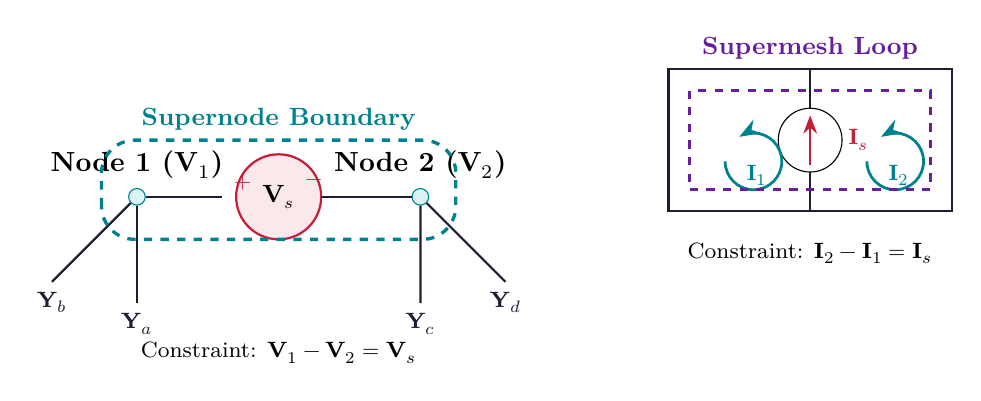
\begin{tikzpicture}[scale=0.9, auto, node distance=2.2cm]
  % Supernode diagram
  \begin{scope}[shift={(0,0)}]
    \node[circnode, label=above:{\textbf{Node 1 ($\mathbf{V}_1$)}}] (n1) at (0,0) {};
    \node[circnode, label=above:{\textbf{Node 2 ($\mathbf{V}_2$)}}] (n2) at (4,0) {};
    
    \draw[line] (n1) -- (1.2,0);
    \draw[draw=myred, fill=hdrred, line width=0.8pt] (2,0) circle (0.6cm) node[font=\small\bfseries] {$\mathbf{V}_s$};
    \node[font=\footnotesize\bfseries, color=myred] at (1.5,0.2) {$+$};
    \node[font=\footnotesize\bfseries, color=myred] at (2.5,0.2) {$-$};
    \draw[line] (2.6,0) -- (n2);
    
    % Branches leaving node 1
    \draw[line] (n1) -- ++(0,-1.5) node[below, font=\footnotesize] {$\mathbf{Y}_a$};
    \draw[line] (n1) -- ++(-1.2,-1.2) node[below, font=\footnotesize] {$\mathbf{Y}_b$};
    
    % Branches leaving node 2
    \draw[line] (n2) -- ++(0,-1.5) node[below, font=\footnotesize] {$\mathbf{Y}_c$};
    \draw[line] (n2) -- ++(1.2,-1.2) node[below, font=\footnotesize] {$\mathbf{Y}_d$};
    
    % Supernode boundary
    \draw[myteal, dashed, line width=1.2pt, rounded corners=12pt] (-0.5,-0.6) rectangle (4.5,0.8);
    \node[color=myteal, font=\small\bfseries] at (2,1.1) {Supernode Boundary};
    \node[font=\footnotesize] at (2,-2.2) {Constraint: $\mathbf{V}_1 - \mathbf{V}_2 = \mathbf{V}_s$};
  \end{scope}

  % Supermesh diagram
  \begin{scope}[shift={(7.5,-0.2)}]
    \draw[line] (0,0) rectangle (4,2);
    \draw[line] (2,0) -- (2,2);
    
    % Current source in shared branch
    \draw[fill=white] (2,1) circle (0.45cm);
    \draw[redarrow] (2,0.65) -- (2,1.35);
    \node[right, font=\footnotesize\bfseries, color=myred] at (2.4,1) {$\mathbf{I}_s$};
    
    % Mesh currents
    \draw[-Stealth, color=myteal, line width=1pt] (0.8,0.7) arc (-180:120:0.4cm) node[midway, left, font=\footnotesize\bfseries] {$\mathbf{I}_1$};
    \draw[-Stealth, color=myteal, line width=1pt] (2.8,0.7) arc (-180:120:0.4cm) node[midway, left, font=\footnotesize\bfseries] {$\mathbf{I}_2$};
    
    % Supermesh boundary
    \draw[mypurple, dashed, line width=1.2pt] (0.3,0.3) -- (3.7,0.3) -- (3.7,1.7) -- (0.3,1.7) -- cycle;
    \node[color=mypurple, font=\small\bfseries] at (2,2.3) {Supermesh Loop};
    \node[font=\footnotesize] at (2,-0.6) {Constraint: $\mathbf{I}_2 - \mathbf{I}_1 = \mathbf{I}_s$};
  \end{scope}
\end{tikzpicture}
\end{tcolorbox}

\subsection{Matrix Mesh (Loop) Impedance Formulation}
For a planar network with $M$ independent meshes, Kirchhoff's Voltage Law (KVL) around clockwise mesh currents yields:
\begin{equation}
  [\mathbf{Z}] \mathbf{I}_m = \mathbf{V}_e
\end{equation}
where:
\begin{equation}
  \begin{bmatrix}
    Z_{11} & Z_{12} & \cdots & Z_{1M} \\
    Z_{21} & Z_{22} & \cdots & Z_{2M} \\
    \vdots & \vdots & \ddots & \vdots \\
    Z_{M1} & Z_{M2} & \cdots & Z_{MM}
  \end{bmatrix}
  \begin{bmatrix}
    \mathbf{I}_1 \\ \mathbf{I}_2 \\ \vdots \\ \mathbf{I}_M
  \end{bmatrix}
  =
  \begin{bmatrix}
    \mathbf{V}_{e1} \\ \mathbf{V}_{e2} \\ \vdots \\ \mathbf{V}_{eM}
  \end{bmatrix}
\end{equation}

\begin{tcolorbox}[formulabox, title={\textbf{Inspection Rules for Mesh Impedance Matrix $[\mathbf{Z}]$}}]
For planar networks with independent voltage sources and passive impedances:
\begin{itemize}[leftmargin=*, itemsep=2pt]
  \item \textbf{Self-Impedance ($Z_{ii}$):} Total sum of all branch impedances forming mesh $i$: $Z_{ii} = \sum Z_{loop\,i}$.
  \item \textbf{Mutual Impedance ($Z_{ij}, i \ne j$):} Negative of the branch impedance common to both mesh $i$ and mesh $j$ when mesh currents flow in opposite directions through the shared branch: $Z_{ij} = -Z_{shared}$.
  \item \textbf{Source Vector ($\mathbf{V}_{ei}$):} Algebraic sum of all independent voltage sources encountered in mesh $i$ clockwise (a potential rise yields positive $\mathbf{V}_e$, a potential drop yields negative $\mathbf{V}_e$).
\end{itemize}
\end{tcolorbox}

\begin{tcolorbox}[defbox, title={\textbf{Supermesh Technique (Current Sources Shared Between Meshes)}}]
When an ideal current source is shared between two adjacent meshes $i$ and $j$:
\begin{enumerate}[leftmargin=*, itemsep=2pt, topsep=1pt]
  \item \textbf{Avoid Shared Branch:} Create a \textbf{supermesh} by conceptually removing the branch containing the current source (leaving an open-circuit path).
  \item \textbf{Apply KVL:} Write one single KVL equation around the combined outer perimeter loop of both meshes.
  \item \textbf{Constraint Equation:} Relate the mesh currents to the current source: $\mathbf{I}_j - \mathbf{I}_i = \mathbf{I}_s$.
\end{enumerate}
\end{tcolorbox}

% ───────────────────────────────────────────────────────────────────────────────
\section{Source Transformation and Network Duality}
% ───────────────────────────────────────────────────────────────────────────────

\subsection{AC Source Transformation}
Any practical AC voltage source consisting of an ideal phasor source $\mathbf{V}_s$ in series with internal impedance $\mathbf{Z}_s$ can be transformed into an equivalent practical AC current source consisting of phasor source $\mathbf{I}_s$ in parallel with internal admittance $\mathbf{Y}_s = 1/\mathbf{Z}_s$:
\begin{equation}
  \mathbf{I}_s = \frac{\mathbf{V}_s}{\mathbf{Z}_s}, \qquad \mathbf{Z}_s = \frac{1}{\mathbf{Y}_s}
\end{equation}
This equivalence holds strictly for all external load terminals at angular frequency $\omega$.

\subsection{Network Duality Principles}
Two networks $N_1$ and $N_2$ are said to be \textbf{dual} to each other if the mesh equations of $N_1$ are mathematically identical in form to the node equations of $N_2$. Duality is an exact topological and algebraic reflection:

\par\vspace{6pt}\noindent
\begingroup
\setlength{\tabcolsep}{6pt}
\setlength{\extrarowheight}{3pt}
\renewcommand{\arraystretch}{1.35}
\begin{tabularx}{\linewidth}{|B{4.5cm}|B{4.5cm}|Y|}
\hline
\multicolumn{1}{|c|}{\textbf{Primary Network Concept}} & \multicolumn{1}{c|}{\textbf{Dual Network Concept}} & \multicolumn{1}{c|}{\textbf{Mathematical Relation}} \\
\hline
Mesh / Loop & Node / Node-Pair & Mesh Current $\mathbf{I}_m \longleftrightarrow$ Node Voltage $\mathbf{V}_n$ \\
\hline
Voltage Law (KVL: $\sum \mathbf{V} = 0$) & Current Law (KCL: $\sum \mathbf{I} = 0$) & Dual equations exchange $V \leftrightarrow I$ \\
\hline
Series Connection & Parallel Connection & $Z = Z_1 + Z_2 \longleftrightarrow Y = Y_1 + Y_2$ \\
\hline
Resistance $R$ ($\Omega$) & Conductance $G$ ($\text{S}$) & $G = R / R_0^2$ (normalized) \\
\hline
Inductance $L$ ($\text{H}$) & Capacitance $C$ ($\text{F}$) & Numerical value: $C = L / R_0^2$ \\
\hline
Voltage Source $\mathbf{V}_s$ & Current Source $\mathbf{I}_s$ & Direction maps clockwise loop $\leftrightarrow$ node entry \\
\hline
Short Circuit ($\mathbf{Z}=0$) & Open Circuit ($\mathbf{Y}=0$) & $\mathbf{V}=0 \longleftrightarrow \mathbf{I}=0$ \\
\hline
\end{tabularx}
\endgroup

\begin{tcolorbox}[tikzbox, title={\textbf{TikZ Schematic: Dual Network Construction on Planar Graphs}}]
\centering
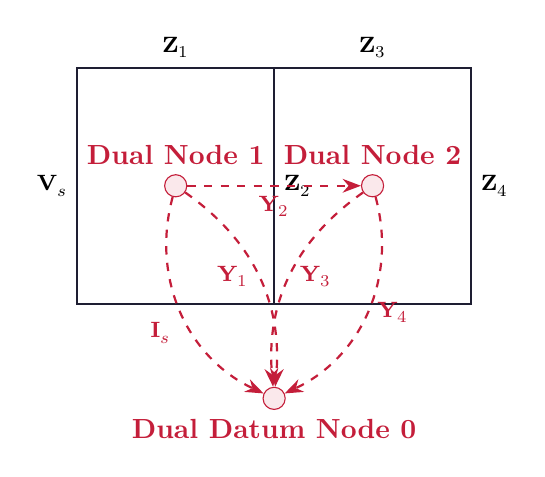
\begin{tikzpicture}[scale=1.0, auto, node distance=2.5cm]
  % Original planar network (Black/Dark lines)
  \draw[line, thick] (0,0) rectangle (5,3);
  \draw[line, thick] (2.5,0) -- (2.5,3);
  
  \node[above, font=\footnotesize\bfseries] at (1.25,3) {$\mathbf{Z}_1$};
  \node[above, font=\footnotesize\bfseries] at (3.75,3) {$\mathbf{Z}_3$};
  \node[left, font=\footnotesize\bfseries] at (0,1.5) {$\mathbf{V}_s$};
  \node[right, font=\footnotesize\bfseries] at (2.5,1.5) {$\mathbf{Z}_2$};
  \node[right, font=\footnotesize\bfseries] at (5,1.5) {$\mathbf{Z}_4$};
  
  % Dual nodes (Red dots in each mesh + 1 outer datum node)
  \node[circle, draw=myred, fill=hdrred, inner sep=2pt, minimum size=8pt, label=above:{\color{myred}\textbf{Dual Node 1}}] (d1) at (1.25,1.5) {};
  \node[circle, draw=myred, fill=hdrred, inner sep=2pt, minimum size=8pt, label=above:{\color{myred}\textbf{Dual Node 2}}] (d2) at (3.75,1.5) {};
  \node[circle, draw=myred, fill=hdrred, inner sep=2pt, minimum size=8pt, label=below:{\color{myred}\textbf{Dual Datum Node 0}}] (d0) at (2.5,-1.2) {};
  
  % Dual branches (Red dashed lines crossing each original branch)
  \draw[redarrow, dashed] (d1) -- (d2) node[midway, below, font=\footnotesize\bfseries] {$\mathbf{Y}_2$};
  \draw[redarrow, dashed] (d1) to[bend left=30] node[left, font=\footnotesize\bfseries] {$\mathbf{Y}_1$} (d0);
  \draw[redarrow, dashed] (d1) to[bend right=40] node[below left, font=\footnotesize\bfseries] {$\mathbf{I}_s$} (d0);
  \draw[redarrow, dashed] (d2) to[bend left=40] node[right, font=\footnotesize\bfseries] {$\mathbf{Y}_4$} (d0);
  \draw[redarrow, dashed] (d2) to[bend right=30] node[right, font=\footnotesize\bfseries] {$\mathbf{Y}_3$} (d0);
\end{tikzpicture}
\end{tcolorbox}

% ───────────────────────────────────────────────────────────────────────────────
\section{Network Theorems as Applied to AC Circuits}
% ───────────────────────────────────────────────────────────────────────────────

\subsection{Superposition Theorem (AC Form)}

\begin{tcolorbox}[defbox, title={\textbf{Superposition Theorem Statement}}]
In any linear, bilateral AC electrical network containing multiple independent sources operating at identical or differing frequencies, the steady-state phasor response (current or voltage) in any branch equals the algebraic sum of the individual phasor responses produced by each independent source acting alone, with all other independent sources set to zero:
\begin{itemize}[leftmargin=*, itemsep=2pt, topsep=1pt]
  \item Independent voltage sources are replaced by short circuits ($\mathbf{V}_s = 0$).
  \item Independent current sources are replaced by open circuits ($\mathbf{I}_s = 0$).
  \item Dependent sources remain untouched and active throughout the procedure.
\end{itemize}
\end{tcolorbox}

\begin{tcolorbox}[examplebox, title={\textbf{Critical Exam Caveat: Superposition with Differing Frequencies and AC Power}}]
\textbf{1. Multi-Frequency Superposition:} If sources operate at distinct angular frequencies ($\omega_1 \ne \omega_2$), phasors \textbf{cannot} be added algebraically in the frequency domain because they exist on different complex bases. Responses must be calculated individually as time functions and summed in the time domain:
\begin{equation}
  v(t) = v_1(t) + v_2(t) = V_{m1} \cos(\omega_1 t + \phi_1) + V_{m2} \cos(\omega_2 t + \phi_2)
\end{equation}
\textbf{2. Average Power is Non-Linear:} Superposition does \textbf{not} hold for power ($P \ne P_1 + P_2$) when sources share the same frequency, because $P \propto I^2 = (I_1 + I_2)^2 = I_1^2 + I_2^2 + 2 I_1 I_2$. Only when sources have orthogonal frequencies ($\omega_1 \ne \omega_2$) does the cross-product average to zero, allowing:
\begin{equation}
  P_{\text{avg}} = P_1 + P_2 \qquad (\text{strictly for } \omega_1 \ne \omega_2)
\end{equation}
\end{tcolorbox}

\subsection{Thevenin's and Norton's Theorems (AC Form)}

\begin{tcolorbox}[defbox, title={\textbf{Thevenin's and Norton's AC Theorems}}]
\textbf{Thevenin's Theorem:} Any linear, bilateral, active two-terminal AC network can be replaced at its external load terminals ($A$-$B$) by an equivalent circuit consisting of an open-circuit phasor voltage source $\mathbf{V}_{th}$ connected in series with an internal equivalent impedance $\mathbf{Z}_{th}$.

\textbf{Norton's Theorem:} The same two-terminal AC network can alternatively be replaced by an ideal short-circuit phasor current source $\mathbf{I}_N$ connected in parallel with an internal equivalent admittance $\mathbf{Y}_N = 1/\mathbf{Z}_{th}$.
\end{tcolorbox}

\begin{tcolorbox}[formulabox, title={\textbf{Analytical Formulation and Evaluation of $\mathbf{V}_{th}, \mathbf{I}_N$ and $\mathbf{Z}_{th}$}}]
\begin{itemize}[leftmargin=*, itemsep=2pt]
  \item \textbf{Open-Circuit Voltage ($\mathbf{V}_{th}$):} $\mathbf{V}_{th} = \mathbf{V}_{oc} = \mathbf{V}_A - \mathbf{V}_B$ across open terminals $A$-$B$.
  \item \textbf{Short-Circuit Current ($\mathbf{I}_N$):} $\mathbf{I}_N = \mathbf{I}_{sc}$ flowing from terminal $A$ to $B$ when short-circuited.
  \item \textbf{Source Inter-relation:} $\mathbf{V}_{th} = \mathbf{I}_N \cdot \mathbf{Z}_{th}$.
  \item \textbf{Evaluation of $\mathbf{Z}_{th}$ (Networks with Dependent Sources):} Deactivate all independent sources. Apply an external test source $\mathbf{V}_{\text{test}}$ across terminals $A$-$B$ and compute resulting input current $\mathbf{I}_{\text{test}}$:
  \begin{equation}
    \mathbf{Z}_{th} = \frac{\mathbf{V}_{\text{test}}}{\mathbf{I}_{\text{test}}} = \frac{\mathbf{V}_{oc}}{\mathbf{I}_{sc}}
  \end{equation}
\end{itemize}
\end{tcolorbox}

\subsection{Maximum Power Transfer Theorem in AC Circuits}
Let a linear AC source be represented by its Thevenin equivalent ($\mathbf{V}_{th}, \mathbf{Z}_{th} = R_{th} + jX_{th}$) driving a complex load impedance $\mathbf{Z}_L = R_L + jX_L$.

\begin{tcolorbox}[formulabox, title={\textbf{Derivation: Condition for Maximum Average Power Transfer}}]
The phasor current through the load is:
\begin{equation}
  \mathbf{I}_L = \frac{\mathbf{V}_{th}}{\mathbf{Z}_{th} + \mathbf{Z}_L} = \frac{\mathbf{V}_{th}}{(R_{th} + R_L) + j(X_{th} + X_L)}
\end{equation}
The magnitude of the load current squared is:
\begin{equation}
  |\mathbf{I}_L|^2 = \frac{|\mathbf{V}_{th}|^2}{(R_{th} + R_L)^2 + (X_{th} + X_L)^2}
\end{equation}
The real average power dissipated in load resistance $R_L$ is:
\begin{equation}
  P_L = |\mathbf{I}_L|^2 R_L = \frac{|\mathbf{V}_{th}|^2 R_L}{(R_{th} + R_L)^2 + (X_{th} + X_L)^2}
\end{equation}
\textbf{Step 1: Optimization with respect to $X_L$:}
To maximize $P_L$, the denominator must be minimized. Setting $\frac{\partial P_L}{\partial X_L} = 0$:
\begin{equation}
  X_L + X_{th} = 0 \implies \mathbf{X}_L = -\mathbf{X}_{th}
\end{equation}
The load reactance must cancel the source reactance (conjugate match condition).

\textbf{Step 2: Optimization with respect to $R_L$:}
With $X_L = -X_{th}$, $P_L = \frac{|\mathbf{V}_{th}|^2 R_L}{(R_{th} + R_L)^2}$. Setting $\frac{dP_L}{dR_L} = 0$:
\begin{equation}
  \frac{d}{dR_L}\left[ \frac{R_L}{(R_{th} + R_L)^2} \right] = \frac{(R_{th} + R_L)^2 - 2R_L(R_{th} + R_L)}{(R_{th} + R_L)^4} = 0 \implies \mathbf{R}_L = \mathbf{R}_{th}
\end{equation}
Combining both conditions yields the \textbf{Complex Conjugate Match}:
\begin{equation}
  \mathbf{Z}_L = R_{th} - jX_{th} = \mathbf{Z}_{th}^*
\end{equation}
The corresponding maximum average power delivered to the load is:
\begin{equation}
  P_{\max} = \frac{|\mathbf{V}_{th}|^2 R_{th}}{(2R_{th})^2} = \frac{|\mathbf{V}_{th}|^2}{4 R_{th}}
\end{equation}
\end{tcolorbox}

\subsubsection{Constrained Load Cases}
\begin{enumerate}[leftmargin=*, itemsep=2pt]
  \item \textbf{Load Phase Angle Fixed ($\mathbf{Z}_L = |Z_L|\angle \theta_L$ with variable magnitude):}
  \begin{equation}
    |Z_L| = |Z_{th}| = \sqrt{R_{th}^2 + X_{th}^2}
  \end{equation}
  \item \textbf{Purely Resistive Load ($X_L = 0, R_L$ variable):}
  \begin{equation}
    R_L = |\mathbf{Z}_{th}| = \sqrt{R_{th}^2 + X_{th}^2}
  \end{equation}
  \item \textbf{Fixed Reactance $X_L$ with Variable Resistance $R_L$:}
  \begin{equation}
    R_L = \sqrt{R_{th}^2 + (X_{th} + X_L)^2}
  \end{equation}
\end{enumerate}

\subsection{Reciprocity Theorem}

\begin{tcolorbox}[defbox, title={\textbf{Reciprocity Theorem in AC Networks}}]
In any linear, bilateral, passive, time-invariant AC network, if an ideal voltage source $\mathbf{V}_1$ applied in branch 1 produces a current $\mathbf{I}_2$ in branch 2, then the same voltage source transferred to branch 2 will produce identical current $\mathbf{I}_1 = \mathbf{I}_2$ in branch 1:
\begin{equation}
  \mathbf{Z}_{12} = \frac{\mathbf{V}_1}{\mathbf{I}_2} = \frac{\mathbf{V}_2}{\mathbf{I}_1} = \mathbf{Z}_{21}
\end{equation}
The transfer impedance is completely symmetrical ($\mathbf{Z}_{12} = \mathbf{Z}_{21}$).
\end{tcolorbox}
\par\vspace{4pt}\noindent
\textbf{Restrictions:} The network must contain no dependent sources, no unilateral devices (like diodes), and only a single source must be active.

\subsection{Compensation (Substitution) Theorem}
If the impedance of a branch carrying steady-state phasor current $\mathbf{I}$ changes by an increment $\Delta\mathbf{Z}$ (from $\mathbf{Z}$ to $\mathbf{Z} + \Delta\mathbf{Z}$), the incremental change in currents and voltages throughout all other branches in the network can be calculated by replacing the altered impedance with a virtual compensation voltage source $\mathbf{V}_c$:
\begin{equation}
  \mathbf{V}_c = \mathbf{I}' \Delta\mathbf{Z} \approx \mathbf{I} \Delta\mathbf{Z}
\end{equation}
directed in opposition to the original current $\mathbf{I}$, while deactivating all original independent sources.

\subsection{Tellegen's Theorem}

\begin{tcolorbox}[defbox, title={\textbf{Tellegen's Theorem}}]
For any lumped electrical network containing $b$ branches and $n$ nodes, whose branch voltages $v_k(t)$ satisfy KVL and branch currents $i_k(t)$ satisfy KCL under associated reference directions:
\begin{equation}
  \sum_{k=1}^b v_k(t) i_k(t) = 0 \qquad \text{at every instant } t
\end{equation}
In the frequency domain for AC steady-state sinusoidal circuits:
\begin{equation}
  \sum_{k=1}^b \mathbf{V}_k \mathbf{I}_k^* = 0 \implies \sum_{k=1}^b P_k + j \sum_{k=1}^b Q_k = 0
\end{equation}
The sum of complex powers delivered to all branches is identically zero (conservation of both active power $P$ and reactive power $Q$).
\end{tcolorbox}

\textbf{Remarkable Scope:} Tellegen's theorem is completely independent of the nature of the network components. It holds whether elements are linear, non-linear, passive, active, time-varying, or time-invariant; it relies solely on the topological graph properties governed by KVL and KCL.

\newpage
% ===============================================================================
% MANDATORY QUICK REVISION PAGE
% ===============================================================================
\begin{center}
  {\large\bfseries\color{myred} Quick Revision --- Module 1}\\[3pt]
  {\small\color{mydark} Mesh, Nodal Analysis and AC Network Theorems $|$ EC304}
\end{center}
\noindent{\color{myred}\rule{\linewidth}{1.2pt}}
\vspace{4pt}

\begin{tcolorbox}[formulabox, title={\textbf{Key Formulas and Network Relations at a Glance}}]
\renewcommand{\arraystretch}{1.35}
\begin{tabularx}{\linewidth}{B{5.0cm} X}
Inductive Reactance & $X_L = \omega L, \quad \mathbf{Z}_L = j\omega L = \omega L \angle 90^\circ$ \\[4pt]
Capacitive Reactance & $X_C = \frac{1}{\omega C}, \quad \mathbf{Z}_C = \frac{-j}{\omega C} = \frac{1}{\omega C} \angle -90^\circ$ \\[4pt]
Nodal Admittance Matrix & $[\mathbf{Y}]\mathbf{V}_n = \mathbf{I}_s, \quad Y_{ii} = \sum y_{branch}, \quad Y_{ij} = -y_{ij}$ \\[4pt]
Mesh Impedance Matrix & $[\mathbf{Z}]\mathbf{I}_m = \mathbf{V}_e, \quad Z_{ii} = \sum Z_{loop}, \quad Z_{ij} = -Z_{shared}$ \\[4pt]
Source Transformation & $\mathbf{I}_s = \mathbf{V}_s / \mathbf{Z}_s, \quad \mathbf{Z}_s = 1 / \mathbf{Y}_s$ \\[4pt]
Maximum Power Condition (AC) & $\mathbf{Z}_L = \mathbf{Z}_{th}^* = R_{th} - jX_{th}$ \\[4pt]
Maximum Power Formula & $P_{\max} = \frac{|\mathbf{V}_{th}|^2}{4 R_{th}} \quad (\text{W})$ \\[4pt]
Resistive Load Max Power & $R_L = |\mathbf{Z}_{th}| = \sqrt{R_{th}^2 + X_{th}^2}$ \\[4pt]
Reciprocity Transfer Symmetry & $\mathbf{Z}_{12} = \frac{\mathbf{V}_1}{\mathbf{I}_2} = \frac{\mathbf{V}_2}{\mathbf{I}_1} = \mathbf{Z}_{21}$ \\[4pt]
Tellegen's Complex Conservation & $\sum_{k=1}^b \mathbf{V}_k \mathbf{I}_k^* = 0 \iff \sum P_k = 0 \text{ and } \sum Q_k = 0$ \\[4pt]
\end{tabularx}
\end{tcolorbox}

\begin{tcolorbox}[defbox, title={\textbf{One-Line Definitions}}]
\begin{itemize}[leftmargin=*, itemsep=2pt, topsep=0pt]
  \item \textbf{Phasor:} A complex representation of a sinusoidal voltage or current containing amplitude and phase angle.
  \item \textbf{Impedance ($\mathbf{Z}$):} Total opposition offered by a network element to sinusoidal alternating current, measured in ohms.
  \item \textbf{Admittance ($\mathbf{Y}$):} The measure of ease with which an AC circuit allows current to flow, defined as $1/\mathbf{Z}$.
  \item \textbf{Supernode:} A generalized node created by enclosing a voltage source connected between two non-reference nodes.
  \item \textbf{Supermesh:} A combined loop formed by avoiding a branch containing an ideal current source shared between two meshes.
  \item \textbf{Dual Networks:} Two networks whose loop equations in one are structurally and mathematically identical to the node equations in the other.
  \item \textbf{Thevenin Equivalent:} An AC circuit reduction consisting of an open-circuit voltage $\mathbf{V}_{th}$ in series with $\mathbf{Z}_{th}$.
  \item \textbf{Norton Equivalent:} An AC circuit reduction consisting of a short-circuit current $\mathbf{I}_N$ in parallel with $\mathbf{Z}_{th}$.
  \item \textbf{Conjugate Match:} Setting load impedance equal to the complex conjugate of source impedance for maximum power transfer.
  \item \textbf{Tellegen's Theorem:} A topological theorem stating that the sum of power delivered over all branches in any lumped network is zero.
\end{itemize}
\end{tcolorbox}

\begin{tcolorbox}[exambox, title={\textbf{Frequently Asked / Viva Questions}}]
\begin{enumerate}[topsep=0pt, label=\textbf{Q\arabic*.}, itemsep=5pt]
  \item \Q{State the condition for maximum power transfer in an AC circuit with complex source and load impedances.}
  Maximum active power transfer occurs when the load impedance is the complex conjugate of the Thevenin impedance: $\mathbf{Z}_L = \mathbf{Z}_{th}^* = R_{th} - jX_{th}$. Under this condition, reactive power cancels out, and $P_{\max} = \frac{|\mathbf{V}_{th}|^2}{4 R_{th}}$.

  \item \Q{Why can the superposition theorem not be directly applied to calculate total AC power?}
  Because power is a non-linear quadratic function of voltage and current ($P = I^2 R$). The square of a sum contains cross-product terms: $(I_1 + I_2)^2 = I_1^2 + I_2^2 + 2 I_1 I_2 \ne I_1^2 + I_2^2$. Therefore, currents or voltages must be superposed first, and power calculated subsequently from the net total.

  \item \Q{How do you evaluate Thevenin impedance $\mathbf{Z}_{th}$ in a circuit containing dependent sources?}
  Deactivate all independent sources (short voltage sources, open current sources). Connect a fictitious test source $\mathbf{V}_{\text{test}}$ across the open terminals, determine the resulting current $\mathbf{I}_{\text{test}}$ supplied by the test source, and compute $\mathbf{Z}_{th} = \mathbf{V}_{\text{test}} / \mathbf{I}_{\text{test}}$.

  \item \Q{What are the fundamental requirements for the Reciprocity theorem to hold in a network?}
  The network must be linear, passive, time-invariant, bilateral, and contain no dependent sources or non-linear elements. Only a single excitation source must be active at a time.

  \item \Q{What is the physical meaning of Tellegen's theorem in an AC circuit?}
  It proves that in any lumped network, the sum of all instantaneous branch powers equals zero. In AC circuits, this implies the simultaneous conservation of both active real power ($\sum P_k = 0$) and reactive imaginary power ($\sum Q_k = 0$).

  \item \Q{When is a supernode required in nodal analysis?}
  When an ideal voltage source (independent or dependent) is connected directly between two non-reference nodes without any series impedance, making the branch current indeterminate from node voltages alone.

  \item \Q{Explain the concept of duality in electrical networks.}
  Two planar networks are duals if the KVL loop equations of one match the KCL node equations of the other. Series branches map to parallel branches, meshes map to nodes, inductors map to capacitors, and voltage sources map to current sources.

  \item \Q{If the load is purely resistive ($X_L = 0$), what is the condition for maximum power transfer from an AC source?}
  The load resistance must equal the magnitude of the source Thevenin impedance: $R_L = |\mathbf{Z}_{th}| = \sqrt{R_{th}^2 + X_{th}^2}$.

  \item \Q{Can Tellegen's theorem be applied to non-linear and time-varying circuits?}
  Yes. Tellegen's theorem depends strictly on Kirchhoff's laws (KVL and KCL), which stem solely from topology (conservation of energy and charge). It holds irrespective of whether elements are linear, non-linear, active, passive, or time-varying.

  \item \Q{What is the difference between Mesh Analysis and Loop Analysis?}
  A mesh is a loop that does not contain any other loops within it (applicable strictly to planar circuits). Loop analysis can be applied to arbitrary closed paths and non-planar networks using fundamental loop sets.
\end{enumerate}
\end{tcolorbox}

\begin{tcolorbox}[tikzbox, title={\textbf{Summary Matrix: Comprehensive Comparison of AC Network Theorems}}]
\par\vspace{4pt}\noindent
\begingroup
\setlength{\tabcolsep}{4.5pt}
\setlength{\extrarowheight}{3pt}
\renewcommand{\arraystretch}{1.35}
\begin{tabularx}{\linewidth}{|B{3.2cm}|B{3.5cm}|Y|}
\hline
\multicolumn{1}{|c|}{\textbf{Theorem}} & \multicolumn{1}{c|}{\textbf{Primary Condition}} & \multicolumn{1}{c|}{\textbf{Practical Applications and Limitations}} \\
\hline
Superposition & Linear, bilateral elements & Multi-frequency circuits; invalid for power calculations. \\
\hline
Thevenin's & Linear active two-terminal & Simplifies terminal analysis; $\mathbf{Z}_{th}$ needs test source if dependent sources exist. \\
\hline
Norton's & Dual of Thevenin's theorem & Current-driven systems; relates via $\mathbf{V}_{th} = \mathbf{I}_N \mathbf{Z}_{th}$. \\
\hline
Maximum Power Transfer & Source $\mathbf{Z}_{th}$ fixed, load adjustable & Conjugate match $\mathbf{Z}_L = \mathbf{Z}_{th}^*$; efficiency is strictly $50\%$. \\
\hline
Reciprocity & Linear, bilateral, passive, no dependent sources & Symmetrical transfer impedance; useful in antennas and filters. \\
\hline
Tellegen's & Any lumped network obeying KVL \& KCL & Holds for linear/non-linear, active/passive; confirms energy conservation. \\
\hline
\end{tabularx}
\endgroup
\end{tcolorbox}

\end{document}
